% XeLaTeX can use any Mac OS X font. See the setromanfont command below.
% Input to XeLaTeX is full Unicode, so Unicode characters can be typed directly into the source.

% The next lines tell TeXShop to typeset with xelatex, and to open and save the source with Unicode encoding.

%!TEX TS-program = xelatex
%!TEX encoding = UTF-8 Unicode

\documentclass[10pt, twocolumn]{article}
\renewcommand{\refname}{\fontsize{10pt}{10pt}\selectfont\textbf{參考文獻}}
\renewcommand{\figurename}{圖}
\usepackage{geometry}                % See geometry.pdf to learn the layout options. There are lots.
\geometry{a4paper, margin=1in}                   % ... or a4paper or a5paper or ... 
%\geometry{landscape}                % Activate for for rotated page geometry
\usepackage[parfill]{parskip}    % Activate to begin paragraphs with an empty line rather than an indent
\usepackage{graphicx}
\usepackage{amssymb}
\usepackage{fancyvrb}
\usepackage{hyperref}
\usepackage{pstricks,pst-node,pst-tree}
\usepackage{rotating}


\usepackage[boldfont,slantfont,CJKnumber,CJKspace]{xeCJK}
\usepackage{CJKnumb}
\setmainfont{Times New Roman}
\setCJKmainfont{cwTeX Q Ming Medium}                                                                 %設定中文預設字體
\setCJKsansfont{cwTeX Q Kai Medium}
	

\XeTeXlinebreaklocale "zh"
\XeTeXlinebreakskip = 0pt plus 1pt


\pagestyle{empty}

\title{\fontsize{14pt}{14pt}\textbf{跨平台軟體持續整合樣式之已知案例探討\\On the known use of a collection of Patterns for Continuous Integration in Cross-Platform Software Development}}
\author{\fontsize{12pt}{12pt}王熙鈞$\dagger$\hspace{3em}謝金雲$\dagger$$\dagger$\hspace{3em}鄭有進$\dagger$$\dagger$\hspace{3em}陳建村$\ddag$\\國立臺北科技大學資訊工程系$\dagger$,$\dagger$$\dagger$\hspace{1em}美超微電腦股份有限公司$\ddag$\\Si-Jyun Wang, Yu Chin Cheng, Chin-Yun Hsieh, and Chien-Tsun Chen\\Department of Computer Science and Information Engineering, \\National Taipei University of Technology$\dagger$,$\dagger$$\dagger$\hspace{1em}Super Micro Computer, Inc. Taiwan$\ddag$\\Email: t7598052@ntut.edu.tw$\dagger$\hspace{1em}$\{$hsieh,yccheng$\}$@csie.ntut.edu.tw$\dagger$$\dagger$\hspace{1em}ctchen@ctchen.idv.tw$\ddag$}
\date{}

%%定義環境變數與巨集指令
%-------------------基本設定------------------------------------%
% 沿用 latex 的一些標點的轉換,如 en-dash 以兩個減號表示
\defaultfontfeatures{Mapping=tex-text}
\XeTeXlinebreaklocale "zh"
\XeTeXlinebreakskip = 0pt plus 1pt
%-------------------------------------------------------------%

%-------------------重新定義章節名稱格式--------------------------%

\titleformat{\chapter}[hang]{\centering\huge\bfseries}{第\CJKnumber{\thechapter}章}{1em}{}
%\renewcommand\chaptername{Chapter\hspace{.5em}\thechapter}
\renewcommand\contentsname{目錄}
\renewcommand\listfigurename{圖目錄}
\renewcommand\listtablename{表目錄}

\titlecontents{chapter}[0pt]{}
    {第\CJKnumber{\thecontentslabel}章\quad}{}
    {\hspace{.5em}\titlerule*[10pt]{$\cdot$}\contentspage}
\titlecontents{section}[2em]{}
    {\thecontentslabel\quad}{}
    {\hspace{.5em}\titlerule*[10pt]{$\cdot$}\contentspage}
\titlecontents{subsection}[4em]{}
    {\thecontentslabel\quad}{}
    {\hspace{.5em}\titlerule*[10pt]{$\cdot$}\contentspage}

% \renewcommand{\refname}{參考文獻}
\renewcommand{\bibname}{參考文獻}			%修改參考文獻的標題名
\titlespacing{\chapter}{0pt}{*0}{*4}		%設定標題與四周的距離
\titlelabel{\thetitle\quad}				%設定章節標題的樣式
\renewcommand{\figurename}{圖}
\renewcommand{\tablename}{表}
%-----------------------------------------------------------------%

%-------------------設定行距--------------------------------------%
\renewcommand{\baselinestretch}{1.6}
%\linespread{1.6}
%設定enumerate等的item間距

%-----------------------------------------------------------------%

%-------------------定義浮水印------------------------------------%
\newcommand\WatermarkPicture{%
   \put(0,0){%
   \parbox[b][\paperheight]{\paperwidth}{%
     \vfill
     \centering
     \includegraphics[width=5cm,keepaspectratio]{watermark_ntut.png}%
     \vfill
     }
   }
}

%-----------------------------------------------------------------%

%------------------圖片巨集---------------------------------------%

%巨集格式
%mygraphic{圖片KeyWord}{圖片註解}{圖片路徑}
\def\myGraphic#1#2#3
{
	\begin{figure}[!htbp]
		\begin{center}
			\includegraphics[width=\textwidth]{#3}
			\caption{#2}\label{#1}
		\end{center}
		
	\end{figure}
}
%-----------------------------------------------------------------%

%------------------小小圖片巨集---------------------------------------%

%巨集格式
%mygraphic{圖片KeyWord}{圖片註解}{圖片路徑}
\def\myGraphicSS#1#2#3
{
	\begin{figure}[!htbp]
		\begin{center}
			\includegraphics[width=2cm]{#3}
			\caption{#2}\label{#1}
		\end{center}
		
	\end{figure}
}
%-----------------------------------------------------------------%

%------------------小圖片巨集---------------------------------------%

%巨集格式
%mygraphic{圖片KeyWord}{圖片註解}{圖片路徑}
\def\myGraphicS#1#2#3
{
	\begin{figure}[!htbp]
		\begin{center}
			\includegraphics[width=6cm]{#3}
			\caption{#2}\label{#1}
		\end{center}
		
	\end{figure}
}
%-----------------------------------------------------------------%

%------------------中圖片巨集---------------------------------------%

%巨集格式
%mygraphic{圖片KeyWord}{圖片註解}{圖片路徑}
\def\myGraphicM#1#2#3
{
	\begin{figure}[!htbp]
		\begin{center}
			\includegraphics[width=8cm]{#3}
			\caption{#2}\label{#1}
		\end{center}
		
	\end{figure}
}
%-----------------------------------------------------------------%

%------------------大圖片巨集---------------------------------------%

%巨集格式
%mygraphic{圖片KeyWord}{圖片註解}{圖片路徑}
\def\myGraphicB#1#2#3
{
	\begin{figure}[!htbp]
		\begin{center}
			\includegraphics[width=12cm]{#3}
			\caption{#2}\label{#1}
		\end{center}
		
	\end{figure}
}
%-----------------------------------------------------------------%

%------------------大大圖片巨集---------------------------------------%

%巨集格式
%mygraphic{圖片KeyWord}{圖片註解}{圖片路徑}
\def\myGraphicBB#1#2#3
{
	\begin{figure}[!htbp]
		\begin{center}
			\includegraphics[width=16cm]{#3}
			\caption{#2}\label{#1}
		\end{center}
		
	\end{figure}
}
%-----------------------------------------------------------------%

%------------------表格巨集---------------------------------------%
\renewcommand{\arraystretch}{1}

%巨集格式
%myTable{Table KeyWord}{Table註解}
\def\myTable#1#2
{
	\begin{table}[!htbp]
	\setlength{\abovecaptionskip}{0pt}
	\setlength{\belowcaptionskip}{10pt}
	\begin{center}
	\caption{#2}\label{#1}
}


\def\endmyTable
{
	\end{center}
	\end{table}
}

%-----------------------------------------------------------------%

%------------------修改圖與表的註解編號格式-----------------------%

\makeatletter
\long\def\@makecaption#1#2{%
  \vskip\abovecaptionskip
  \sbox\@tempboxa{{\bfseries #1}\quad #2}%
  \ifdim \wd\@tempboxa >\hsize
    {\bfseries #1}\quad #2\par
  \else
    \global \@minipagefalse
    \hb@xt@\hsize{\hfil\box\@tempboxa\hfil}%
  \fi
  \vskip\belowcaptionskip}
\makeatother


%-----------------------------------------------------------------%
%------------------修改Description縮排格式--------------------------%
%\makeatletter
%\renewenvironment{description}
%  {\list{}{\leftmargin\z@ \labelwidth\z@ \itemindent-\leftmargin
%   \let\makelabel\descriptionlabel}}
%  {\endlist}
%\makeatother
%-----------------------------------------------------------------%
%------------------Use Case巨集---------------------------------------%
%巨集格式
%useCase{UseCase名稱}{UseCase圖片路徑}
\def\useCase#1#2#3
{
	\subsection{#1}
	\begin{figure}[!htb]
		\begin{center}
			\includegraphics[width=\textwidth]{#2}
		\end{center}
	\end{figure}
}
% \graphicspath{{./picture/eps/}{./picture/png/}}
\graphicspath{{.}}					%告訴Latex去這兩個目錄下找圖檔
%-----------------------------------------------------------------%
%-------------------為了方便所設定的巨集--------------------------%

%-----------------------------------------------------------------%


\begin{document}
\maketitle
\thispagestyle{empty}


%\fontsize{10pt}{12pt}\selectfont
%\textbf{\begin{center}摘要\end{center}}

\begin{center}\textbf{摘要}\end{center}

\parindent=2em軟體開發團隊實踐持續整合,藉此順利完成軟體開發,這是軟體開發業界多年來的共識。目前已有跨平台軟體持續整合樣式語言被整理提出,用以協助軟體開發團隊在開發跨平台軟體時實踐持續整合。雖然這些跨平台軟體持續整合樣式語言是以特定領域的跨平台軟體專案實踐持續整合的經驗為基礎,但要真正成為一個樣式語言,其中之樣式需要有更多的實例。
本論文以開放原始碼的跨平台軟體專案\textendash\hspace{4pt}Chromium作為案例探討的對象,並提出探討已知案例之研究方法,利用該方法尋找已知案例。本論文於實例中已找到了四個樣式的已知案例,足以說明跨平台軟體持續整合樣式語言的有效性。

\textbf{關鍵詞:}\fontsize{9pt}{9pt}\selectfont 跨平台軟體開發、持續整合、樣式語言、樣式
\fontsize{10pt}{12pt}\selectfont

\begin{raggedright}\textbf{1. 緒論}\end{raggedright}

\parindent=2em開發跨平台軟體是一項於技術面、商業策略上都極具挑戰的工作。為了達成軟體於不同平台上運行的目標,軟體公司Netscape定義其瀏覽器軟體為跨平台軟體,並基於同一份程式碼,同時為了不同平台使用者開發瀏覽器產品。由上述經驗可知開發跨平台軟體的困難如下所述,撰寫跨平台程式碼必須留意各個平台上的特性,再來應該減少專屬於特定平台的原始碼,最後於不同平台上執行測試將更加耗時\cite{netscapecrossplatform}。雖然該公司最終因為軟體生命週期管理不當、微軟競逐瀏覽器市場等因素,而逐漸式微,但是該公司對於跨平台軟體開發的經驗依然值得借鏡。

持續整合論述發展一個產品,無論是軟硬體,都不能將整合工作延遲至專案開發階段的末期才開始進行,所以必須於專案初期就進行整合,並且在交付產品前都不能停止。基於這樣的精神,注重及早交付產品的敏捷式軟體開發流程將持續整合視為最佳實踐。在執行持續整合時,首重確實實行各種必須涵蓋於其中的步驟,例如為了維持軟體系統品質,於整合流程中,敏捷式軟體開發團隊涵蓋各種驗證軟體品質的步驟。此外相關經驗如何於團隊成員間傳遞,亦為實踐持續整合必須考慮的事項,例如執行持續整合流程時各種錯誤排除的經驗。在市面上有許多持續整合的工具,然而工具並無法傳達如何實踐持續整合。軟體開發團隊若未體悟工具無法根除執行持續整合本質上的問題,且團隊未建立起積極面對整合議題的態度,持續整合將淪為形式。

跨平台軟體開發團隊執行持續整合流程,用以降低於不同平台上進行測試的成本。於持續整合流程中必須涵蓋各種形式的自動化測試,這樣的作法將對跨平台軟體開發帶來衝擊,因為於持續整合流程中,執行過多的測試將造成開發團隊簽入原始碼的過程冗長,如此間接使得團隊成員執行持續整合的意願降低\cite{teampace}。面對上述的問題,開發團隊由自身累積的經驗中找到解決方法,不僅可以應用於本身的專案,尚可與其他開發團隊分享這些經驗,以幫助其他開發團隊執行持續整合。

C.-Y. Hsieh等提出跨平台軟體持續整合樣式語言\cite{crossplatformcipatterns},並以正規形式呈現其中樣式,期望跨平台軟體開發團隊利用該樣式語言,順利實踐持續整合,藉此完成跨平台軟體之開發。 雖然藉由特定領域軟體開發實踐持續整合的經驗,C.-Y. Hsieh等累積該經驗形成跨平台軟體持續整合樣式語言,但是尚需要更多的實例來實證C.-Y. Hsieh等提出的樣式語言之真實性與有效性。本論文以軟體建置、檔案目錄結構、架構設計、專案社群文件四個構面為途徑探討開放原始碼專案Chromium,期望於其中得到跨平台軟體持續整合樣式之已知案例,用以確定樣式語言存在之真實性與其有效性。 %此外藉由跨平台軟體開發團隊對於實踐持續整合的經驗與知識,輔以他人已經發表過持續整合樣式,將合適的樣式與經驗融入跨平台軟體持續整合樣式語言中,進一步演化此一樣式語言。

\parindent=2em本論文分成四個章節。第一章為緒論,介紹研究背景與動機、研究目標、論文組織與架構。第二章為背景介紹,介紹關於跨平台軟體開發、持續整合與跨平台軟體持續整合樣式語言等知識。第三章為實例介紹,針對跨平台開放原始碼軟體專案Chromium\cite{chromiumproject} ,就跨平台軟體持續整合樣式語言的Project範疇,尋找個別樣式的已知案例。第四章為結論,介紹本論文的貢獻。

\begin{raggedright}\textbf{2. 背景介紹}\end{raggedright}

\parindent=2em各小節分別介紹跨平台軟體開發、持續整合與跨平台軟體持續整合樣式語言。

\begin{raggedright}\textbf{2.1 跨平台軟體開發}\end{raggedright}

\parindent=2em舉瀏覽器軟體為例,說明開發跨平台軟體的目的。為了要滿足不同平台上瀏覽網路的使用者,所以各家瀏覽器供應商除了微軟以外\footnote{因為搭載視窗作業系統的上網裝置還是達到80\%以上的市占率。\cite{osmarketshare}},都將其自家產品定義為跨平台軟體,期望可以提高在瀏覽器市場的市占率。瀏覽器軟體的problem domain\cite{problemdomain}是網際網路應用與HTML等規格,這些規格無關於平台特性,但是瀏覽器供應商必須同時於多個平台上開發同一個產品。

\parindent=2em開發跨平台軟體的挑戰,主要分成設計面、需求面與流程面三方面介紹。在設計面,應該把與平台相關的程式碼分離開,並提供一個抽象化介面來封裝與平台相關的實作,其他與平台無關的程式碼相依於此介面,而不是個別平台的實作\cite{gofdesignpattern}\cite{slogan}。在需求面上,開發者必須面對在A平台上可以輕易實作出來的功能,在B平台上卻無法以相同方法實現之困境。此外為了避免相依只能於特定平台上運行的API X,開發者必須使用由團隊設計於各個平台通用的介面,但是上述只限定於某平台的API X卻能提供最佳效能。於該平台上,此限制導致跨平台軟體的執行效能較其他可以運用API X的軟體稍差\cite{netscapecrossplatform}。在流程面,開發人員於不同平台上撰寫程式碼,並將程式碼簽入同一程式碼版本控制系統中,開發者A因為撰寫適用於特定平台的程式碼,而造成軟體無法在其他平台建置,該開發者在不知情的狀況下簽入版本控制系統,最後導致其他開發者無法進行開發工作。此外必須時常對多平台進行測試,需要耗費倍數於對單一平台測試的資源進行測試\cite{netscapecrossplatform}。

\begin{raggedright}\textbf{2.2 持續整合}\end{raggedright}

對於執行整合工作,軟體工程師往往無法準確估計時程,這是因為個別模組可以獨立地正常運作,但是和其他模組整合在一起時,整個軟體系統卻無法運作。因為整合工作擁有上述特性,所以整合工作也具備高風險特性,通常在接近軟體釋出的階段,軟體工程師才開始進行整合工作,這代表一旦有整合失敗的情形發生將有無數的修正必須進行,延期釋出軟體是難以避免的。風險越高的工作需要越早、越頻繁被執行,持續整合概念主張以自動化的方式對於軟體進行編譯、測試、靜態分析、產生可交付產品的流程、產出對於程式碼進行測試後的報表,並且在一天當中進行不只一次的整合工作,用以分散、降低執行整合工作的風險,進而有效減輕軟體開發風險。當執行整合工作的頻率增加,即新的程式碼簽入版本控制系統中即執行一次整合工作,而且在軟體開發週期中沒有停止並永續地被執行,如此的頻繁程度則可以稱為持續,若軟體開發團隊落實上述的實踐,則宣稱該團隊實踐持續整合。此外任何使建置整合工作出現錯誤的情況,即可稱為發生Broken Build,當上述情形發生時,軟體開發團隊必須儘早排除狀況,以維護軟體的整體品質。

持續整合可以紓緩開發跨平台軟體時,對於流程面的衝擊。每一次程式碼簽入版本控制系統,必須進行一次整合,並且在所有預定要佈屬的平台上都進行整合,強迫開發團隊儘早解決整合過程發生的問題。即早解決問題,有助於開發工作的進展。於各個平台上,跨平台軟體開發團隊進行測試所衍生的總成本以數量A表示,開發非跨平台軟體的測試成本以數量B表示,數量A是數量B的許多倍,上述情況是開發跨平台軟體時的主要問題,所以整合過程必須包含自動化的測試,藉助自動化測試的幫助得以有效降低成本。

軟體開發團隊執行持續整合除了依賴工具,用以執行自動化的建置與驗證流程外,尚需要落實各種最佳實務。Martin Fowler於\cite{continuousintegration2007} \textendash\hspace{3pt}導讀中提到執行持續整合會對軟體開發流程造成副作用,而軟體開發團隊會因為副作用而放棄實踐持續整合,並且提示軟體開發團隊落實持續整合除了借重工具輔助外,尚需要實踐各種最佳實務,才能使得軟體開發團隊繼續實踐持續整合,並達成持續整合的永續執行特性。樣式語言可以描述落實最佳實務之經驗與知識。

%\begin{raggedright}\textbf{2.3 樣式語言}\end{raggedright}

%\parindent=2em對於樣式的定義,節錄A Pattern Language(1977)\cite{apatternlanguage}一書關於樣式的定義\footnote{請見該本書序言的第10頁},來做說明。

 %\textit{“The elements of the language are entities called patterns. Each pattern describes a problem which occurs over and over again in our environment, and then describes the core of the solution to the problem, in such a way that you can use this solution a million times over, without ever doing it the same way twice.”}

%所以,樣式是針對特定情境下,所發生問題的解法,而且是可以被重複使用的解法。通常要呈現一個樣式可以用下列形式表達。
%\begin{description}
%\setlength{\parsep}{0ex minus5ex}
%\setlength{\itemsep}{0ex minus5ex}
%\setlength{\topsep}{0ex plus5ex}
%\item Name:樣式命名。
%\item Context:一個情境,於此,樣式為了解決問題被發展。
%\item Forces:於情境中所出現的現象,互相衝突的現象形成問題。
%\item Problem:於情境中出現的問題。
%\item Solution:在特定情境中解決問題的方法。
%\item Resulting Context:解法套用後,情境的描述。
%\item Related Patterns:與樣式相關的其他樣式。
%\end{description}

%\parindent=2em對於樣式與樣式語言之間的關係,舉於The Timeless Way of Building(1979)\cite{thetimelesswayofbuilding}出現的例子\footnote{前見該本書的第313頁},解釋兩個樣式之間有連接關係存在時,此關係的解讀,請見圖1。
%\begin{figure}
%\begin{center}
%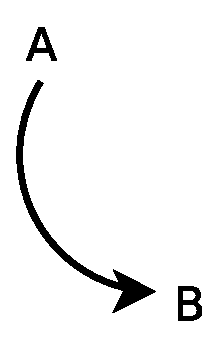
\includegraphics[width=2cm]{pattern-connection.eps}
%\caption{Pattern A 與 Pattern B之間關係解釋圖示}
%\end{center}
%\end{figure}
%Pattern A 如果要解決預定要解的問題,必須依賴Pattern B,Pattern B 解決了一部分Pattern A要解的問題,如果Pattern B未能解決這一部分的問題,Pattern A就無法解決預定要解決的問題。樣式之間存在結構化網絡關係,樣式才可能形成樣式語言。樣式語言可以視為有一個目標、要解決一個規模更大的問題、要平衡為數更多且更加複雜的現象(Forces),處在樣式語言網絡中的樣式,一同解決樣式語言要解決的問題,最後平衡Forces。
 
\begin{raggedright}\textbf{2.3 跨平台軟體持續整合樣式語言}\end{raggedright}

\parindent=2em因為期望傳達開發跨平台軟體時實踐持續整合的知識與經驗,所以C.-Y. Hsieh等提出跨平台軟體持續整合樣式語言,藉此幫助軟體開發團隊開發跨平台軟體。跨平台軟體持續整合樣式語言,將樣式分成三大範疇,分別是Project, Build, Good Habit。可以將此三大範疇之樣式建立網絡關係,形成樣式語言\footnote{Good Habit範疇只有一個樣式,基本上無法稱為一個樣式語言,後續工作將演化Good Habit 範疇樣式語言形成一個形式上與功能上完整的樣式語言。}。三大類樣式語言要解決的問題分別為。
\begin{enumerate}
\item 軟體開發團隊於開發跨平台軟體時,在實踐持續整合的前提下,如何依照separation of concern和module decomposition的原理\cite{satextbook},將專案分解成數個子專案。
\item 跨平台軟體開發團隊於實踐持續整合時,在避免Broken Build的前提下,如何定義建置軟體的工作流程。
\item 跨平台軟體開發團隊於實踐持續整合時,如何因應Broken Build的發生。
\end{enumerate}
%\begin{figure}
%\begin{center}
%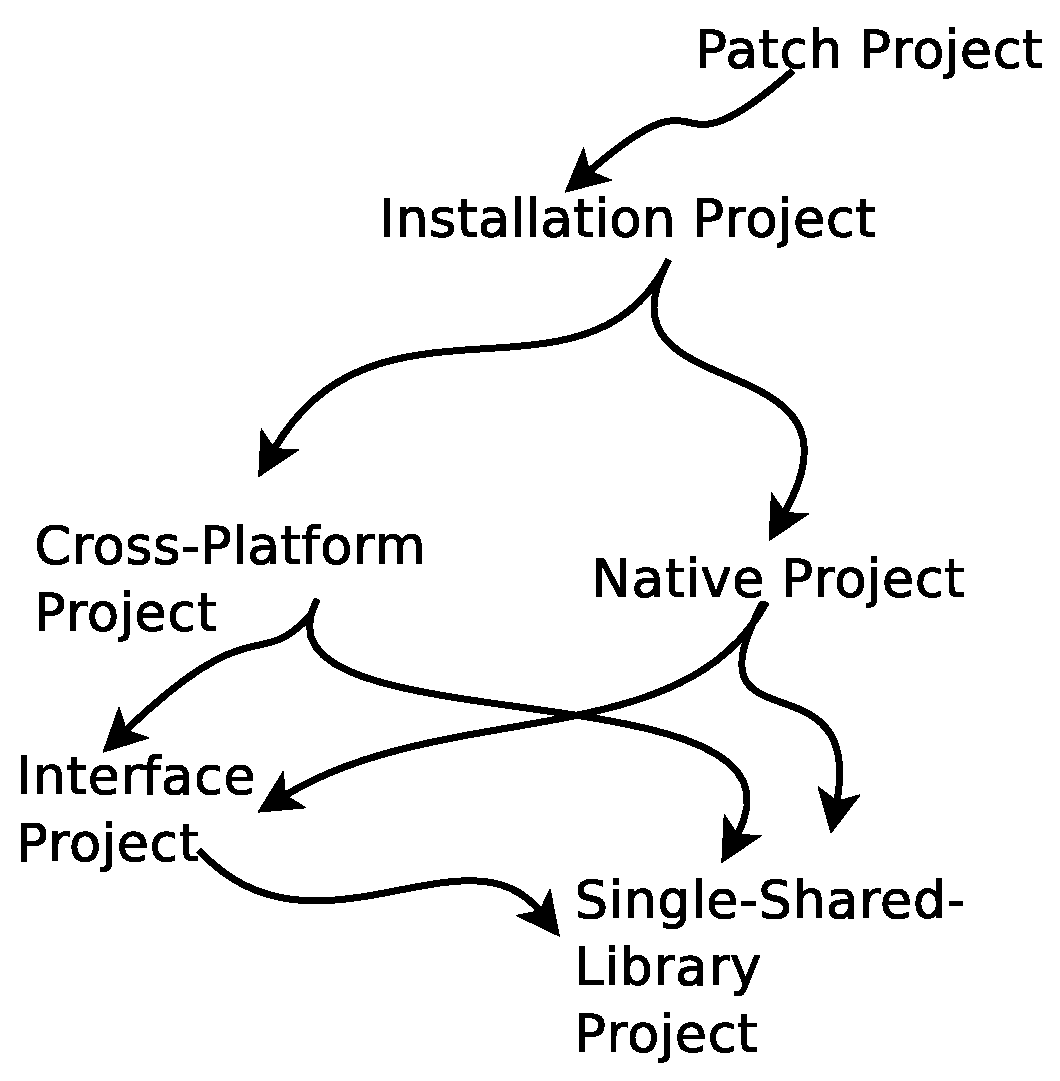
\includegraphics[width=8cm]{project-catgory-pattern-language-network.eps}
%\caption{Project Category 樣式語言網絡圖示}
%\end{center}
%\end{figure}

%\parindent=2em圖2描述Project Category樣式語言網絡關係。僅針對Interface Project, Cross-Platform Project, Native Project, Single Shared Library Project四個樣式之間的關係作說明。
%\begin{description}
%\item Cross-Platform Project與Interface Project的關係:與平台無關的程式碼,必須透過處於Interface Project中的介面定義,間接去使用與平台相關的實作。Cross-Platform Project樣式的功能要趨近完整,必須相依於Interface Project樣式本身的能力。
%\item Native Project與Interface Project的關係:與平台有關的實作程式碼,如果要被平台無關的程式碼所使用,必須依循著介面的定義實作,與平台無關的程式碼才能透過介面使用到這些實作。Native Project樣式的功能要趨近完整,必須相依於Interface Project樣式本身的功能。
%\item Interface Project, Cross-Platform Project, Native Project與Single Shared Library Project的關係:歸屬於上述三種Project的程式碼參考第三方的軟體函式庫時,因為Single Shared Library Project解決了第三方軟體函式庫管理的問題,所以程式碼參考第三方軟體函式庫的問題,必須依賴Single Shared Library樣式提供的能力解決。
%\end{description}
%\begin{figure}
%\begin{center}
%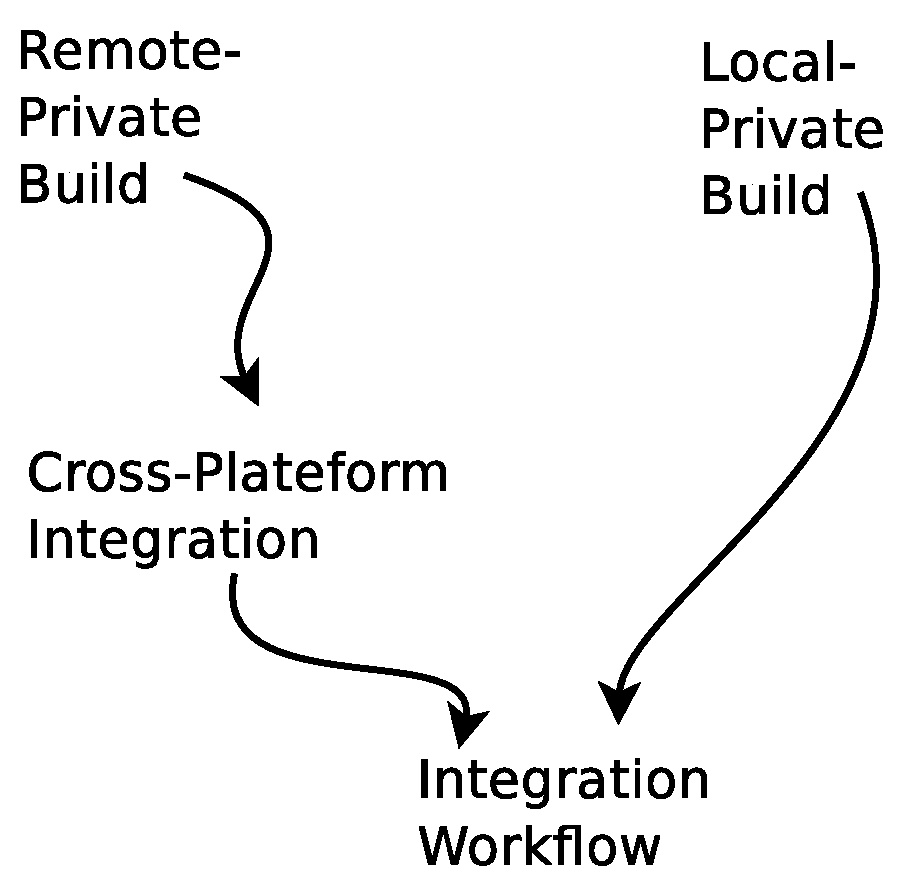
\includegraphics[width=6cm]{build-catgory-pattern-language-network.eps}
%\caption{Build Category 樣式語言網絡圖示}
%\end{center}
%\end{figure}

%\parindent=2em在跨平台軟體持續整合樣式語言提出時,尚未表達Build Category樣式語言網絡關係,本論文提出該樣式語言的網絡關係,請見圖3。Remote Private Build樣式與Cross-Platform Integration樣式有關係。將此關係作為範例說明,Remote Private Build是在原始碼簽入版本控制系統前,開發人員將開發端的原始碼變更置放於持續整合系統進行建置整合流程,此流程必須在所有產品預設要佈署的平台上執行。所以,Remote Private Build樣式要發揮完善功能,必須相依Cross-Platform Integration樣式。

\begin{raggedright}\textbf{3. 跨平台軟體持續整合樣式語言的已知案例}\end{raggedright}

%\textit{In order to discover patterns which are alive we must always start with observation.}
%\begin{flushright}by Christopher Alexander, The Timeless Way of Building(1979), p.254.\end{flushright}
\parindent=2em本章節將以Chromium專案為實例,探索\cite{crossplatformcipatterns}的已知案例。首先本論文提出研究方法,接著再利用該方法探討關於Project範疇樣式語言的已知案例。

\begin{raggedright}\textbf{3.1 研究方法}\end{raggedright}

\parindent=2em本論文以軟體建置、檔案目錄結構、架構設計、專案社群文件等途徑觀察探討樣式的已知案例,請見圖~\ref{observation-view}。%界定專案是此方法主要探討的核心,以不同的構面觀察將得到不同認知。
\begin{description}
\item 軟體建置:軟體建置將原始碼轉換成可執行檔,原始碼依照架構設計被歸類至不同的目錄中。在經過編譯後,隸屬不同子目錄但在概念上合適形成一個元件之程式碼形成元件,上述各個元件以一定順序進行連結將形成最終的可執行檔。因為建置腳本\footnote{Apache Ant build script, Microsoft Visual Studio Solution files, Xcode Project files等皆可歸類為建置腳本。}記錄軟體建置步驟、概念上相近的程式碼形成元件的關係,所以我們不排除藉此找到Installation Project, Patch Project, Native Project, Cross-Platform Project, Interface Project。
\item 檔案目錄結構:依照separation of concern與module decomposition原則,軟體開發團隊將意義上相似、可以聚合形成模組的程式碼分類並置放於不同目錄,所以介面與實作應該置放在不同的目錄。在意義上相似的程式碼所聚集成的目錄,經由此構面觀察可視為一個專案。
\item 架構設計:基於檔案目錄結構構面並考慮架構設計議題,本構面針對處於不同目錄之程式碼所產生的關連加強論述。在設計系統架構時,利用介面分離與平台有關的實作、與平台無關的通用程式碼,分離後上述三種類型的原始碼應該分別置於不同目錄,但並不能強制規範進行分離的作法。但在僅需新增對應平台的實作而不更動介面的前提下,為了方便新增對另一種平台的支援,介面、與平台相關的程式碼必須被強制分離至不同子專案中。
\item 專案社群文件:因為成員分散於世界各地,所以開放原始碼專案社群文件必須記錄有關軟體建置、檔案目錄結構、架構設計等等知識,方便新進成員儘快了解該專案。對於各類討論持續整合相關議題之書籍與網站,以專案社群文件構面進行觀察時,本論文亦將上述內容納入該構面中。
\end{description}

上述四種途徑有互相依賴的現象,實際進行觀察時,觀察者不可能只利用一種途徑探討樣式之已知案例。通常首先從建置軟體的構面進行觀察,因為以持續整合的觀點出發,最直接被關心的是軟體如何被編譯建置。再來我們關注概念上相似的程式碼如何被分類、置放於目錄結構中,於其中可以定位與平台有關、無關之專案。接著我們關注分屬不同類型專案之程式碼間的關連,找尋是否有扮演介面角色之程式碼,並確定該類程式碼、與平台有關之程式碼、與平台無關之程式碼之間的關係,以上描述有賴架構設計構面之觀察才可實現。最後,輔以專案社群文件構面進行觀察,可以補足或加速以上述三種構面進行觀察之不足或進度。

\begin{figure}
\begin{center}
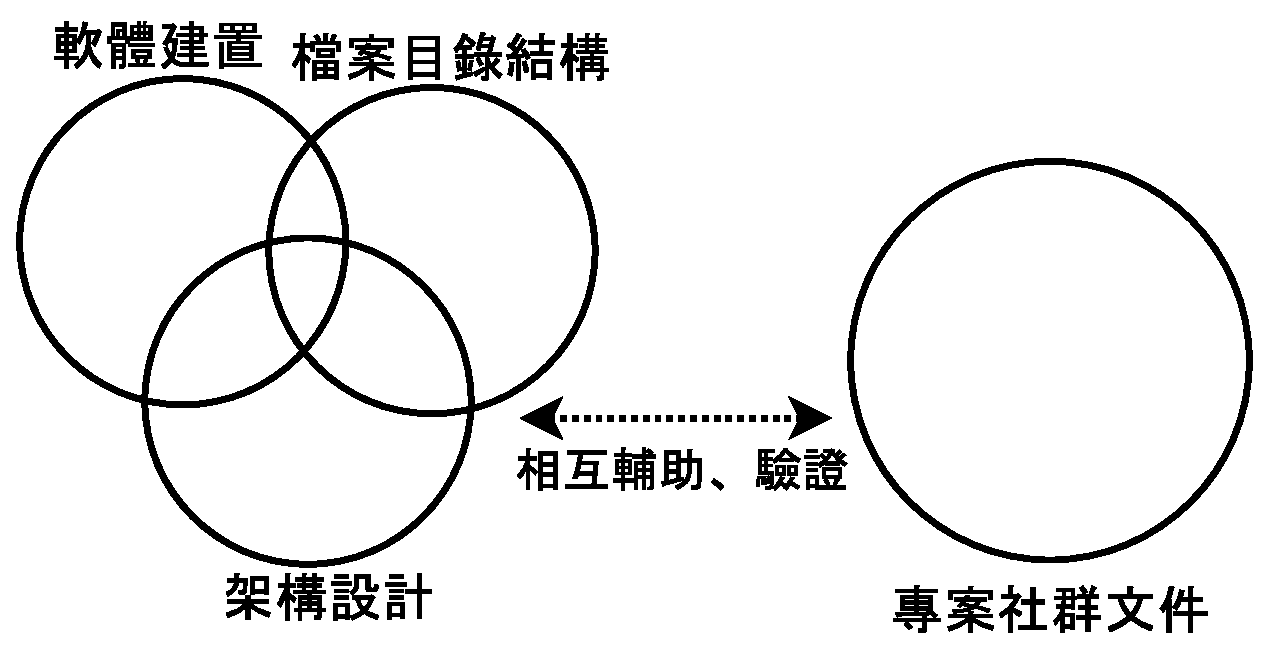
\includegraphics[width=8cm]{observation_view.eps}
\caption{用以觀察已知案例的四個構面}
\label{observation-view}
\end{center}
\end{figure}

\begin{raggedright}\textbf{3.2 探討Project Category樣式語言以Chromium專案為實例}\end{raggedright}

Chromium專案是一個跨平台開放原始碼專案,以C, C++, Objective-C程式語言實作一個Web瀏覽器,主要支援Linux, Mac OS X, Windows等平台,於Mac OS X平台上,與UI相關的程式碼以Objective-C程式語言實作,與其他平台共用之程式碼則使用C, C++程式語言實作。這是由Google所贊助的專案,Google正式釋出的瀏覽器是以Chrome命名,一般來說Chromium會提供比較新穎的功能,這些功能大概一段時間後,Google才會在釋出新版本的Chrome瀏覽器時,將這些功能涵蓋進Chrome的釋出版本中。Google 藉著Chromium專案的成功與成果,已經非常迅速地在瀏覽器市場中,獲得10\%左右的市佔率\cite{browsermarketshare}。

\parindent=2em首先從建置軟體的構面出發進行觀察,於Mac OS X系統上,Chro\-mium\-專案的建置腳本即Xcode IDE專案檔,利用Xcode IDE\cite{xcode}開啟代表實例的主要專案檔案chrome.\-xcode\-project,實際開啟後,發現實例中所有相關的程式碼在Xcode中是以名為chrome的專案涵蓋,發現chrome專案底下有許多子目錄與子專案。各個專案中定義Targets,於其中定義由哪些檔案經過編譯後形成動態連結檔案、執行檔;以下將舉chrome, content子專案為例討論其中的Target,請見圖~\ref{deploymentview-content}與圖~\ref{deploymentview-chrome}。首先討論content子專案,置放於content\-/\textit{Source}\-/\textit{browser}\-, content\-/\textit{Source}\-/\textit{common}\-子目錄中的程式碼,經過編譯形成兩個動態連結檔案libcontent\_browser.a, libcontent\_common.a。以形成一個動態連結檔案的數個原始碼視為一完整概念,則content\-/\textit{Source}\-/\textit{browser}\-, content\-/\textit{Source}\-/\textit{common}\-子目錄視為一專案。再來討論chrome子專案,置放於render\_host, tab\_contents子目錄中的程式碼與其他置放在chrome\-/\textit{Source}\-/\textit{browser}\-目錄底下的程式碼一同編譯形成一可執行檔案,以形成一個可執行檔案的數個原始碼視為一完整概念,則chrome\-/\textit{Source}\-/\textit{browser}\-子目錄視為一專案。

以軟體建置的構面觀察尚無法明確的指出建置順序與子專案間的關係,很難清楚界定與平台有關、無關與提供介面的子專案,所以必須以設計面的觀點輔助探討。此外以此構面觀察所界定的專案,與經由檔案目錄結構與架構設計構面觀察所界定的專案,我們可以預期兩者不一定完全一致。

\begin{figure}
\begin{center}
\includegraphics[width=8cm]{deploymentview.eps}
\caption{以建置軟體的構面觀察content子專案}
\label{deploymentview-content}
\end{center}
\end{figure}

\begin{figure}
\begin{center}
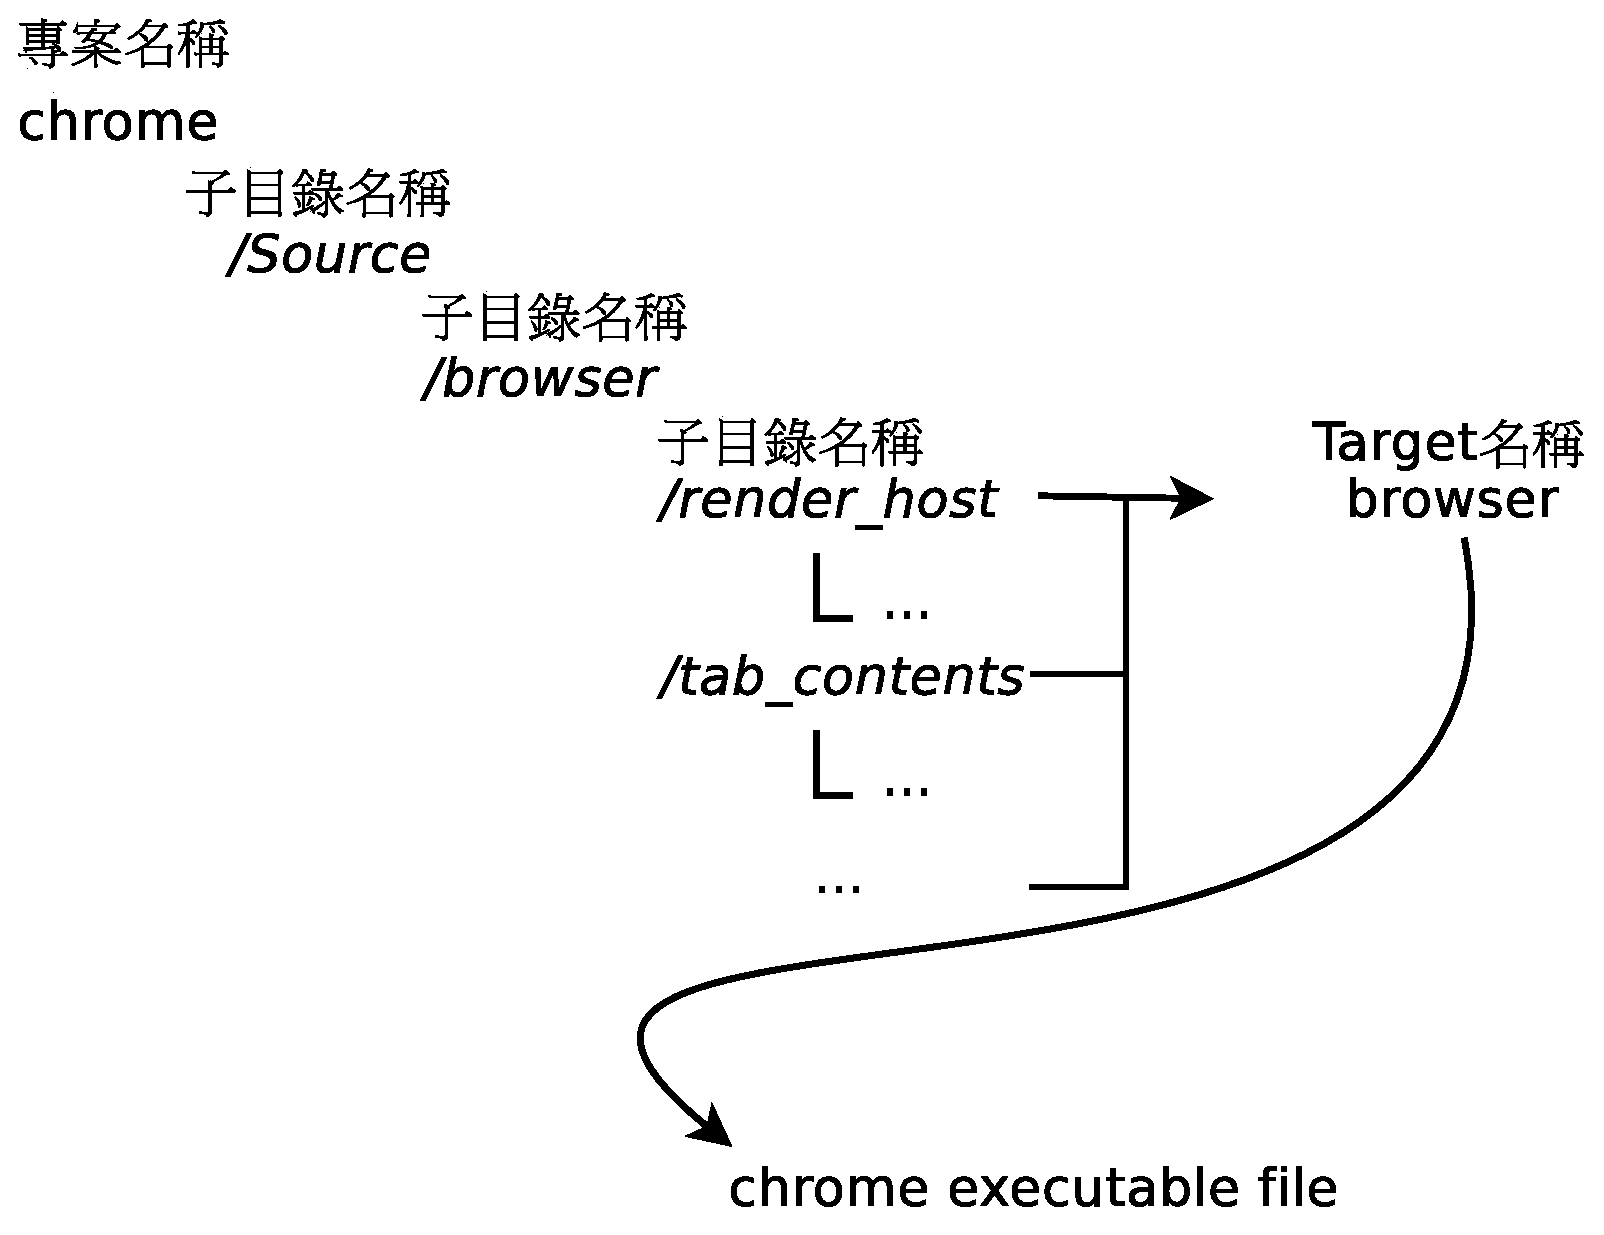
\includegraphics[width=8cm]{deploymentview-chrome.eps}
\caption{以建置軟體的構面觀察chrome子專案}
\label{deploymentview-chrome}
\end{center}
\end{figure}

\begin{figure}
\begin{center}
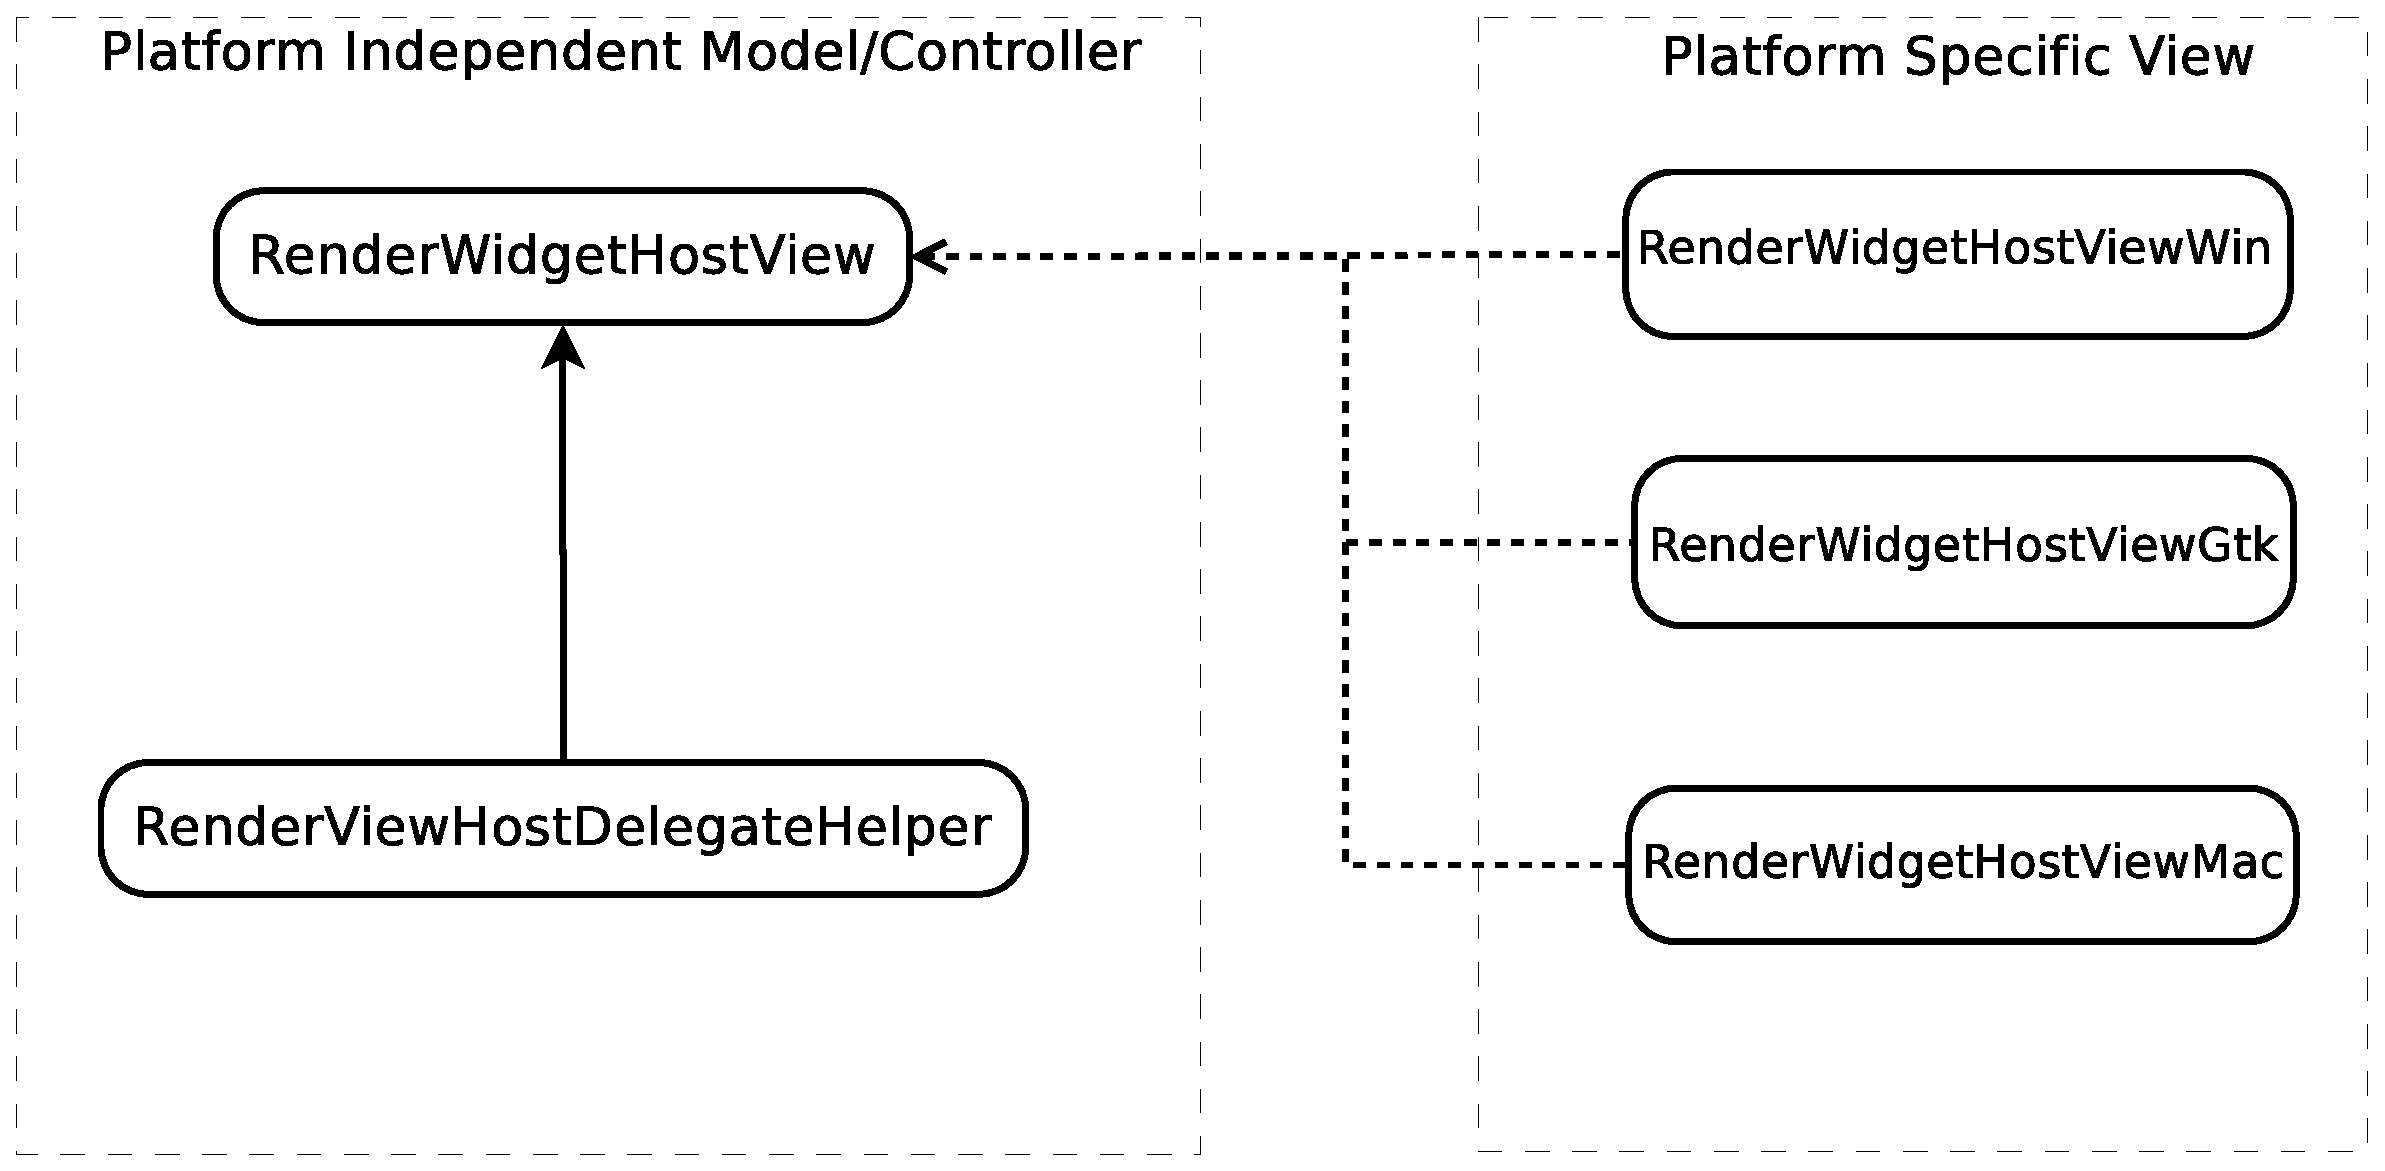
\includegraphics[width=8cm]{chromium-mvc.eps}
\caption{以共同介面建立與平台有關的View}
\label{chromium-mvc}
\end{center}
\end{figure}

%\begin{table}[!htbp]
%\setlength{\abovecaptionskip}{0pt}
%\setlength{\belowcaptionskip}{10pt}
%\begin{tabular}[width=\textwidth]{|c|c|}
%\hline
%\multicolumn{2}{|c|}{專案名稱}\\
%\hline
%\multicolumn{2}{|c|}{chrome}\\
%\hline
%\hline
%\multicolumn{2}{|c|}{\textit{子目錄}}\\
%\hline
%\textit{Source}&\textit{Intermediates}\\
%\hline
%\hline\textit{Product}&\textit{Frameworks}\\
%\hline
%\textit{Projects}&\textit{Build}\\
%\hline
%\hline
%\multicolumn{2}{|c|}{\textit{Projects}子目錄所涵蓋的子專案}\\
%\hline
%base&content\\
%\hline
%WebCore&app\\
%\hline
%Webkit&webkit\\
%\hline
%...&...\\
%\hline
%\end{tabular}
%\label{projectlistview}
%\caption{Chromium專案的子目錄與子專案(70個左右)}
%\label{subprojectfolderview}
%\end{table}


\begin{figure}
\begin{sideways}
	\psscalebox{0.7}{\psset{%linecolor= bisque,%
			nodesep=2pt,%,
			 treemode=D,%
			 levelsep=*1.5cm}
\pstree{\Tr{chrome.xcodeproject}}
			 {\pstree{\Tr{chrome}}{
			    {\pstree{\Tr{\textit{Source}}}
			 	{\pstree{\Tr{\textit{browser}}}
					{\pstree{\Tr{\textit{tab\_contents}}}
					  {\Tr{\underline{render\_view\_host\_delegate\_helper.cc}}
					  }
					  \pstree{\Tr{\textit{render\_host}}}
					  {\Tr{\underline{render\_widget\_host\_view\_*}}
					  }
					  \Tr{...}
					}
				   \Tr{...} 
				}
				
			   }
			 	\pstree{\Tr{content}}
				   {\pstree{\Tr{\textit{Source}}}
					{\pstree{\Tr{\textit{browser}}}
			 			{\pstree{\Tr{\textit{render\_host}}}
					  	{\Tr{\underline{render\_widget\_host\_view.h}}
					  	%{\Tr{render\_widget\_host\_view\_gtk.cc}}
					  	%{\Tr{render\_widget\_host\_view\_mac.mm}}
					  	}
					  	\Tr{...}
					}
				 	{\Tr{...}}
					}
				          \Tr{...}	
				  }
				  
			 \Tr{...}
			 }
			}
			}
\end{sideways}		
\begin{center}
\caption{專案結構與目錄結構 - Chromium,其中子目錄以斜體字體標示,原始碼檔案以底線標示,子專案以正常字體標示。}
\label{fig-folderstructure}
\end{center}
\end{figure}

\begin{figure}
\fontsize{8pt}{8pt}\selectfont
\begin{Verbatim}[numbers=left,framesep=1mm,numbersep=-12pt]
	節錄自render_widget_host_view.h
	// RenderWidgetHostView is an interface 
	// implemented by an object that acts as
	// the "View" portion of a RenderWidgetHost.
	// The RenderWidgetHost and its
	// associated RenderProcessHost own
	// the "Model" in this case which is the
	// child renderer process.
	// The View is responsible for receiving
	// events from the surrounding environment
	// and passing them to the RenderWidgetHost,
	// and for actually displaying the content
	// of the RenderWidgetHost when it changes.
	Class RenderWidgetHostView{
	    public:
	        virtual ~RenderWidgetHostView();
	        
	        // Platform-specific creator.
	        // Use this to construct new 
	        // RenderWidgetHostViews
	        // rather than using 
	        // RenderWidgetHostViewWin 
	        // & friends.
	        ...
	        static RenderWidgetHostView* Create
	            ViewForWidget(RenderWidgetHost
	            View* widget);
	          ...
	  }
\end{Verbatim}
\caption{節錄程式碼 part1: 介面定義}
\label{interfacedef}
\end{figure}

\begin{figure}
\fontsize{8pt}{8pt}\selectfont
\begin{Verbatim}[numbers=left,framesep=1mm,numbersep=-12pt]
	節錄自render_widget_host_view_win.cc 
	RenderWidgetHostView* RenderWidgetHostView
	::CreateViewForWidget(RenderWidgetHostView*
	widget){
	    return new 
	    RenderWidgetHostViewWin(widget);
	}
	節錄程式碼 part2: Windows平台之實作
\end{Verbatim}
\caption{節錄程式碼 part2: Windows平台之實作}
\label{windowsimple}
\end{figure}

\begin{figure}
\fontsize{8pt}{8pt}\selectfont
\begin{Verbatim}[numbers=left,framesep=1mm,numbersep=-12pt]
	節錄自render_widget_host_view_linux.cc
	RenderWidgetHostView* RenderWidgetHostView
	::CreateViewForWidget(RenderWidgetHostView*
	widget){
	    return new 
	    RenderWidgetHostViewGtk(widget);
	}
	節錄程式碼 part3: Linux平台之實作
\end{Verbatim}
\caption{節錄程式碼 part3: Linux平台之實作}
\label{linuximpl}
\end{figure}

\begin{figure}
\fontsize{8pt}{8pt}\selectfont
\begin{Verbatim}[numbers=left,framesep=1mm,numbersep=-12pt]
	節錄自render_widget_host_view_mac.mm
	RenderWidgetHostView* RenderWidgetHostView
	::CreateViewForWidget(RenderWidgetHostView*
	widget){
	    return new 
	    RenderWidgetHostViewMac(widget);
	}
	節錄程式碼 part4: Mac平台之實作
\end{Verbatim}
\caption{節錄程式碼 part4: Mac平台之實作}
\label{macimpl}
\end{figure}

\begin{figure}
\fontsize{8pt}{8pt}\selectfont
\begin{Verbatim}[numbers=left,framesep=1mm,numbersep=-12pt]
	節錄自render_view_host_delegate_helper.cc
	RenderWidgetHostView* RenderViewHostDelegate
	ViewHelper::CreateNewWidget(int route_id, 
	WebKit::WebPopupType popup_type, 
	RenderProcessHost* process) {
	   RenderWidgetHost* widget_host =
	   new RenderWidgetHost(process, route_id);
	   RenderWidgetHostView* widget_view =
	   RenderWidgetHostView::
	   CreateViewForWidget(widget_host);
	   // Popups should not get activated.
	   widget_view->set_popup_type(popup_type);
	   // Save the created widget associated with
	   // the route so we can show it later.
	   pending_widget_views_[route_id] =
	   widget_view;
	   return widget_view;
	}
\end{Verbatim}
\caption{節錄程式碼 part5: 與平台無關之程式碼呼叫介面}
\label{crossplatformcall}
\end{figure}

%\fontsize{10pt}{12pt}\selectfont

\parindent=2em研究Chro\-mium專案網站上的設計文件\cite{chromiummvc},發現Chro\-mium專案在設計上使用Model-View-Controller架構\cite{modelviewcontroller},十分清楚地區分與平台有關的實作、與平台無關的程式碼、介面。圖~\ref{chromium-mvc}表達與View相關的程式碼具有與平台相關的特性,像是專屬於視窗平台之實作Render\-Widget\-Host\-View\-Win,該類別實作於Render\-Widget\-Host\-View定義的介面。如有一與平台無關的程式碼檔案必須參考Render\-Widget\-Host\-View\-Win,必須避免在該程式碼檔案中,撰寫一些判斷不同平台行為的程式碼。因此需要提供一個介面,讓與平台無關的程式碼可以依賴該介面,而不需依賴專屬不同平台的實作。根據這個作法可以在類別Render\-Widget\-Host\-View觀察到介面的存在,而這個類別的定義存在於render\_widget\_host\_view.h中。這個檔案是置放於content子專案中的browser子目錄中的render\_host目錄,請見圖~\ref{fig-folderstructure}。
而對應不同平台的實作如Windows, Linux, Mac\-\ OS\-\ X分別存在render\_\-widget\_\-host\_\-view\_\-win.cc, render\_\-widget\_\-host\_\-view\_\-linux.cc, render\_\-widget\_\-host\_\-view\_\-mac.mm檔案中,請見圖~\ref{windowsimple}, ~\ref{linuximpl}, ~\ref{macimpl}。實作檔案置放於chrome專案中的 browser 目錄底下的render\_host目錄,請見圖~\ref{fig-folderstructure}。
介面指的是Create\-View\-For\-Widget\-(Render\-Widget\-Host* widget)這個Method,請見圖~\ref{interfacedef}的第二十五行,此外請注意該Method是定義為static Method,且亦為Factory Method之實踐\cite{gofdesignpattern},用以抽象化專屬於不同平台之RederWidgetHostView實體的創造過程。
接著,我們發現定義於render\_view\_host\_delegate\_helper.cc的類別Render\-View\-Host\-Delegate\-Helper所包含的Method(Create\-New\-Widget(int route\_id, WebKit::Web\-Popup\-Type popup\_type, Render\-Process\-Host* process))呼叫該介面,介面指的是Render\-Widget\-HostView::Create\-View\-For\-Widget\-(Render\-Widget\-Host* widget),因為CreateViewForWidget(RenderWidgetHost* widget)定義為static,在呼叫該Method時,程式設計師必須連同類別名稱、scope resolution operator(::)、Method名稱一起指定撰寫,請見~\ref{crossplatformcall}第八到十行。該原始碼檔案是一個與平台無關的程式碼,這個檔案是置放於chrome子專案中的browser目錄底下的tab\_contents目錄,請見圖~\ref{fig-folderstructure}。此目錄有置放其他與平台相關的程式碼,依照3.1節 - 檔案目錄結構的描述來進行解讀,因為類別Render\-View\-Host\-Delegate\-Helper在概念意義上,比較接近置放於tab\_contents目錄底下的其他類別,所以還是被置放在tab\_contents目錄底下。此檔案擁有與平台無關的特性,因此將它歸類成與平台無關的程式碼。此外本論文是以補抓某一時間點、快照式的觀點進行觀察,且Chromium專案是一個尚在持續發展的專案,當下與平台無關、相關的程式碼共同置放在同一目錄,但是將來順應架構設計上的改變,而有分離平台無關、相關
程式碼的計畫,針對這點我們並無法排除其可能性,必須長時間加以觀察。

以架構設計、檔案目錄結構構面論述上述觀察的結果,介面定義、實作、與平台無關的程式碼分別被置放%在不同的專案(目錄)中。
content\-/\textit{Source}\-/\textit{browser}\-/\textit{render\_host},%目錄中包含browser控制render的定義,
chrome\-/\textit{Source}\-/\textit{browser}\-/\textit{render\_host},%目錄中包含browser控制render的實作,
chrome\-/\textit{Source}\-/\textit{browser}\-/\textit{tab\_contents}\-目錄中,在上述目錄中分別包含browser控制render的定義、browser控制render的實作、browser將每一個tab中的內容交給render呈現的控制邏輯,在概念上上述三個目錄可分別視為一個模組,或是一個專案,且分別扮演Interface Project, Native Project, Cross-Platform Project的角色,所以上述三個專案(目錄)分別是Interface Project, Native Project, Cross-Platform Project三種樣式的已知案例。

%以軟體建置構面論述上述觀察的結果,介面定義、實作、與平台無關的程式碼分別置放於content\-/\textit{Source}\-/\textit{browser}\-/\textit{render\_host}\-$\dagger$, chrome\-/\textit{Source}\-/\textit{browser}\-/\textit{render\_host}\-$\ddag$, chrome\-/\textit{Source}\-/\textit{browser}\-/\textit{tab\_contents}\-$\ddag$目錄中,上述三個目錄分別被 Target:content\_browser$\dagger$, Target:browser$\ddag$涵蓋。Target:content\_browser, Target:browser對應的子目錄名稱分別為content\-/\textit{Source}\-/\textit{browser}$\dagger$, chrome\-/\textit{Source}\-/\textit{browser}$\ddag$,前者扮演Interface Project$\dagger$、後者扮演Native Project與Cross-Platform Project$\ddag$的角色,所以上述兩個專案(目錄)分別是Interface Project$\dagger$, Native Project與Cross-Platform Project$\ddag$三種樣式的已知案例,請見圖~\ref{chromium-project-category-analysis-view-deploymentview}。

觀察Chromium專案社群文件後,我們發現該專案已經定義各種建置的target,利用Xcode即可進行編譯,並且產生對應不同target的安裝檔案。比如說,對Release target進行編譯建置,即可產出一個專屬於Mac OS X平台的安裝檔案,並且於Mac OS X平台上,針對該安裝檔案進行自動化驗收測試。所以chrome專案是一個Installation Project的已知案例。

在這個實例中,總共找到Interface Project, Cross-Platform Project, Native Project, Installation Project這四個樣式的已知案例,請見圖~\ref{chromium-project-category-analysis-view}。

%\parindent=2em此外,chrome專案已經定義各種建置的target,利用Xcode即可進行編譯,並且產生對應不同target的安裝檔案。比如說,對Release target進行編譯建置,即可產出一個專屬於Mac OS X平台的安裝檔案,並且於Mac OS X平台上,針對該安裝檔案進行自動化驗收測試。所以chrome專案是一個Installation Project的已知案例。
%選擇對Debug target進行編譯建置,產出一個包含Debug Symbol的可執行檔案,方便於執行期間進行除錯。或是

\begin{figure}
\begin{center}
\includegraphics[width=8cm]{chromium-project-category-analysis-view.eps}
\caption{Project Category樣式語言\textendash\hspace{4pt}Chromium版本}
\label{chromium-project-category-analysis-view}
\end{center}
\end{figure}

%\parindent=2em對於3.1節的結論如下。在這個實例中,總共找到Interface Project, Cross-Platform Project, Native Project, Installation Project這四個樣式的已知案例。此外,Chromium專案成員在開發跨平台軟體時,解決類似於Project Category樣式語言所描述的問題,從中得到的經驗與知識,形成了專屬於Chromium專案的樣式語言網絡關係,請見圖4。

%\parindent=0em\textit{“A language is a living language only when each person in society, or in the town, has his own version of this language.” }
%\begin{flushright}by Christopher Alexander, p.337,The timeless way of building(1979).\end{flushright}

%\parindent=0em所以Chromium專案成員對於實踐持續整合,所累積的經驗與知識,形成了自己的樣式語言,雖然沒有完全符合Project Category樣式語言,卻實證了Project Category樣式語言是一個真實存在的樣式語言。

\begin{raggedright}\textbf{4. 結論}\end{raggedright}

\parindent=2em本論文提出探討跨平台軟體持續整合樣式語言的研究方法,並以Chromium為實際案例,探討跨平台軟體持續整合樣式語言的已知案例。自實例中,發現了四個樣式的已知案例,分別為Installation Project, Interface Project, Cross-Platform Project, Native Project。這樣的結果,足以驗證跨平台軟體持續整合樣式語言的有效性。此外由實例中所得到對於實踐持續整合的經驗與知識,有助於演化跨平台軟體持續整合樣式語言。

\begin{raggedright}\textbf{5. 致謝}\end{raggedright}

\parindent=2em本研究接受行政院國家科學委員會計畫99-2221-E-027-096-MY3補助,特此致謝。

\bibliographystyle{plain}
\bibliography{reference}


\end{document}  
